\documentclass[a4paper]{arrowhead}

\usepackage[yyyymmdd]{datetime}
\usepackage{etoolbox}
\usepackage[utf8]{inputenc}
\usepackage{multirow}

\renewcommand{\dateseparator}{-}

\setlength{\parskip}{1em}

%% Special references
\newcommand{\fref}[1]{{\textcolor{ArrowheadBlue}{\hyperref[sec:functions:#1]{#1}}}}
\newcommand{\mref}[1]{{\textcolor{ArrowheadPurple}{\hyperref[sec:model:#1]{#1}}}}
\newcommand{\pdef}[1]{{\textcolor{ArrowheadGrey}{#1\label{sec:model:primitives:#1}\label{sec:model:primitives:#1s}\label{sec:model:primitives:#1es}}}}
\newcommand{\pref}[1]{{\textcolor{ArrowheadGrey}{\hyperref[sec:model:primitives:#1]{#1}}}}

\newrobustcmd\fsubsection[3]{
  \addtocounter{subsection}{1}
  \addcontentsline{toc}{subsection}{\protect\numberline{\thesubsection}interface \textcolor{ArrowheadBlue}{#1}}
  \renewcommand*{\do}[1]{\rref{##1},\ }
  \subsection*{
    \thesubsection\quad
    interface
    \textcolor{ArrowheadBlue}{#1}
    (\notblank{#2}{\mref{#2}}{})
    \notblank{#3}{: \mref{#3}}{}
  }
  \label{sec:functions:#1}
}
\newrobustcmd\msubsection[2]{
  \addtocounter{subsection}{1}
  \addcontentsline{toc}{subsection}{\protect\numberline{\thesubsection}#1 \textcolor{ArrowheadPurple}{#2}}
  \subsection*{\thesubsection\quad#1 \textcolor{ArrowheadPurple}{#2}}
  \label{sec:model:#2} \label{sec:model:#2s} \label{sec:model:#2es}
}
\newrobustcmd\msubsubsection[3]{
  \addtocounter{subsubsection}{1}
  \addcontentsline{toc}{subsubsection}{\protect\numberline{\thesubsubsection}#1 \textcolor{ArrowheadPurple}{#2}}
  \subsubsection*{\thesubsubsection\quad#1 \textcolor{ArrowheadPurple}{#2}}
  \label{sec:model:#2} \label{sec:model:#2s}
}
%%

\begin{document}

%% Arrowhead Document Properties
\ArrowheadTitle{orchestration-service-by-id} % XXX = ServiceName 
\ArrowheadServiceID{orchestration-service-id-proxy} % ID name of service
\ArrowheadType{Service Description}
\ArrowheadTypeShort{SD}
\ArrowheadVersion{4.6.0} % Arrowhead version X.Y.Z, e..g. 4.4.1
\ArrowheadDate{\today}
\ArrowheadAuthor{Rajmund Bocsi} % Corresponding author e.g. Jerker Delsing
\ArrowheadStatus{RELEASE} % e..g. RELEASE, RELEASE CONDIDATE, PROTOTYPE
\ArrowheadContact{rbocsi@aitia.ai} % Email of corresponding author
\ArrowheadFooter{\href{www.arrowhead.eu}{www.arrowhead.eu}}
\ArrowheadSetup
%%

%% Front Page
\begin{center}
  \vspace*{1cm}
  \huge{\arrowtitle}

  \vspace*{0.2cm}
  \LARGE{\arrowtype}
  \vspace*{1cm}

  %\Large{Service ID: \textit{"\arrowid"}}
  \vspace*{\fill}

  % Front Page Image
  %\includegraphics{figures/TODO}

  \vspace*{1cm}
  \vspace*{\fill}

  % Front Page Abstract
  \begin{abstract}
    This document provides service description for the \textbf{orchestration-service-by-id} service. 
  \end{abstract}

  \vspace*{1cm}

%   \scriptsize
%   \begin{tabularx}{\textwidth}{l X}
%     \raisebox{-0.5\height}{
\includegraphics[width=2cm]{figures/artemis_logo}} & {ARTEMIS Innovation Pilot Project: Arrowhead\newline
%     THEME [SP1-JTI-ARTEMIS-2012-AIPP4 SP1-JTI-ARTEMIS-2012-AIPP6]\newline
%     [Production and Energy System Automation Intelligent-Built environment and urban infrastructure for sustainable and friendly cities]}
%   \end{tabularx}
%   \vspace*{-0.2cm}
 \end{center}

\newpage
%%

%% Table of Contents
\tableofcontents
\newpage
%%

\section{Overview}
\label{sec:overview}
This document describes the \textbf{orchestration-service-by-id} service that provides runtime (late) binding between application systems. It is a special version of \textbf{orchestration-service}. Its primary purpose is to provide application systems with orchestration information: where they need to connect to. The outcome of the service includes data that will tell the application system what service provider system(s) it should connect to and how (acting as a service consumer). Such orchestration data include:

\begin{itemize}
    \item Accessibility information details of a service provider (e.g network address and port),
    \item Details of the service instance within the provider system (e.g. base URL, IDD specification and other metadata),
    \item Authorization-related information (e.g. access token and signature),
    \item Additional information that is necessary for establishing connection.
\end{itemize}

The rest of this document is organized as follows.
In Section \ref{sec:functions}, we describe the abstract message functions provided by the service.
In Section \ref{sec:model}, we end the document by presenting the data types used by the mentioned functions.

\subsection{How This Service Is Meant to Be Used}
The given system should consume the Service Registry Core System’s \textbf{query} service to get information about the \textbf{orchestration-service-by-id} service. Using this information the system can request the \textbf{orchestration-service-by-id} service with its own database id. The service returns the top priority local provider of all services contained by the Orchestrator store database for the consumer system.

\subsubsection{The orchestration process}

Figure \ref{fig:activity_uml} describes the orchestration process.

\begin{figure}[h!]
  \centering
  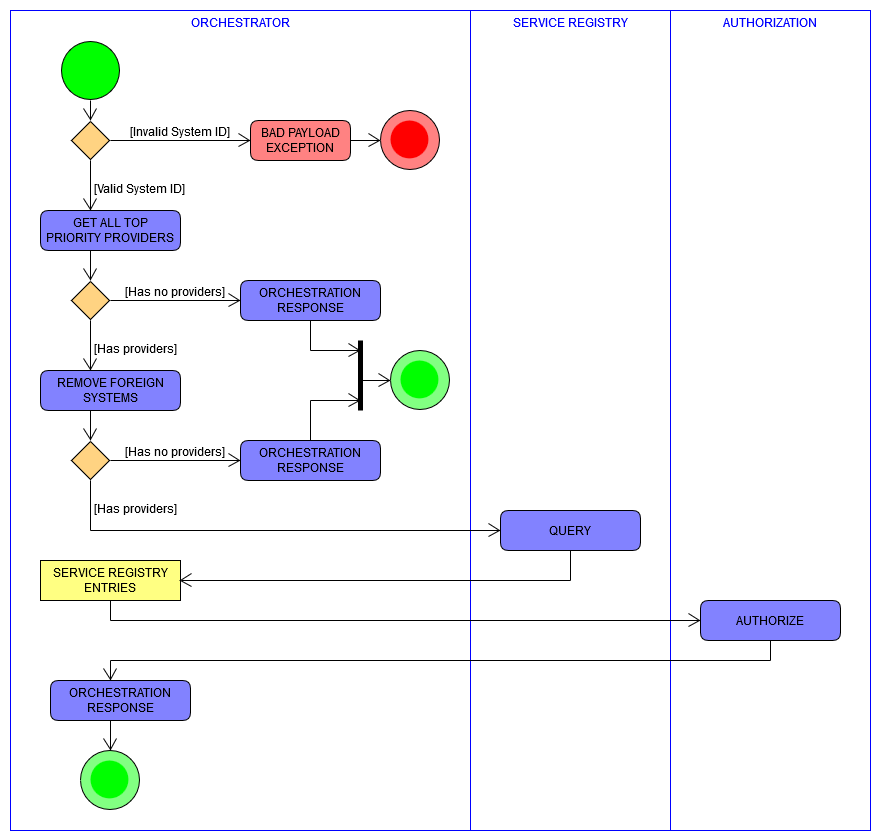
\includegraphics[width=16cm]
  {figures/post_store_orchestration_activity_uml}
  \caption{
    UML activity diagram of the orchestration process.
  }
  \label{fig:activity_uml}
\end{figure}

\clearpage

\subsection{Important Delimitations}
\label{sec:delimitations}

\begin{itemize}
    \item This service is only supports the fix store orchestration.
    \item Inter-cloud rules are not supported.
    \item Orchestration flags are not supported.
    \item Quality-of-Service requirements are not supported.
    \item Provider reservation is not supported.
\end{itemize}

\subsection{Access policy}
\label{sec:accesspolicy}

Available for anyone within the local cloud.

\newpage

\section{Service Interface}
\label{sec:functions}

This section describes the interfaces to the service. The \textbf{orchestration-service-by-id} service is used to looking for matching providers. Each subsection names an interface, an input type and an output type, in that order.
The input type is named inside parentheses, while the output type is preceded by a colon.
Input and output types are only denoted when accepted or returned, respectively, by the interface in question. All abstract data types named in this section are defined in Section 3.

The following interfaces are available.

\fsubsection{HTTP/TLS/JSON}{Number}{OrchestrationResultList}

\begin{table}[ht!]
  \centering
  \begin{tabular}{|l|l|l|l|}
    \rowcolor{gray!33} Profile type & Type & Version \\ \hline
    Transfer protocol & HTTP & 1.1 \\ \hline
    Data encryption & TLS & 1.3 \\ \hline
    Encoding & JSON & RFC 8259 \cite{rfc8259} \\ \hline
    Compression & N/A & - \\ \hline
  \end{tabular}
  \caption{HTTP/TLS/JSON communication details.}
  \label{tab:comunication_semantics_profile}
\end{table}

\clearpage

\section{Information Model}
\label{sec:model}

Here, all data objects that can be part of the \textbf{orchestration-service-by-id} service
provides to the hosting System are listed in alphabetic order.
Note that each subsection, which describes one type of object, begins with the \textit{struct} keyword, which is used to denote a collection of named fields, each with its own data type.
As a complement to the explicitly defined types in this section, there is also a list of implicit primitive types in Section \ref{sec:model:primitives}, which are used to represent things like hashes and identifiers.

\msubsection{struct}{OrchestrationResultList}
\label{sec:model:OrchestrationResultList}

\begin{table}[ht!]
\begin{tabularx}{\textwidth}{| p{3cm} | p{6cm} | X |} \hline
\rowcolor{gray!33} Field & Type & Description \\ \hline
response & \pref{List}$<$\hyperref[sec:model:OrchestrationResult]{OrchestrationResult}$>$ & List of orchestration results. \\ \hline
\end{tabularx}
\end{table}

\msubsection{struct}{OrchestrationResult}
\label{sec:model:OrchestrationResult}

\begin{table}[ht!]
\begin{tabularx}{\textwidth}{| p{4cm} | p{4.6cm} | X |} \hline
\rowcolor{gray!33} Field & Type & Description \\ \hline
authorizationTokens & \hyperref[sec:model:Metadata]{Metadata} & Tokens to use the service instance (one for every supported interface). Only filled if the security type is \texttt{TOKEN}. \\ \hline
interfaces & \pref{List}$<$\hyperref[sec:model:ServiceInterfaceRecord]{ServiceInterfaceRecord}$>$ & List of interfaces the service instance supports. \\ \hline
metadata & \hyperref[sec:model:Metadata]{Metadata} & Service instance metadata. \\ \hline
provider & \hyperref[sec:model:SystemRecord]{SystemRecord} & Descriptor of the provider system record. \\ \hline
secure & \pref{SecureType} & Type of security the service instance uses. \\ \hline
service & \hyperref[sec:model:ServiceDefinitionRecord]{ServiceDefinitionRecord} & Descriptor of the service definition record. \\ \hline
serviceUri & \pref{String} & Path of the service on the provider. \\ \hline
version & \pref{Version} & Version of the service instance. \\ \hline
warnings & \pref{List}$<$\pref{OrchestratorWarning}$>$ & List of warnings about the provider and/or its service instance. \\ \hline
\end{tabularx}
\end{table}

\msubsection{struct}{Metadata}
\label{sec:model:Metadata}

An \pref{Object} which maps \pref{String} key-value pairs.

\clearpage

\msubsection{struct}{ServiceInterfaceRecord}
\label{sec:model:ServiceInterfaceRecord}

\begin{table}[ht!]
\begin{tabularx}{\textwidth}{| p{4.25cm} | p{3.5cm} | X |} \hline
\rowcolor{gray!33} Field & Type & Description \\ \hline
createdAt & \pref{DateTime} & Interface instance record was created at this UTC time\-stamp. \\ \hline
id & \pref{Number} & Identifier of the interface instance. \\ \hline
interfaceName &\pref{Interface} & Specified name of the interface. \\ \hline
updatedAt & \pref{DateTime} & Interface instance record was modified at this UTC time\-stamp. \\ \hline
\end{tabularx}
\end{table}

\msubsection{struct}{SystemRecord}
\label{sec:model:SystemRecord}

\begin{table}[ht!]
\begin{tabularx}{\textwidth}{| p{4.25cm} | p{3.5cm} | X |} \hline
\rowcolor{gray!33} Field & Type & Description \\ \hline

address &\pref{Address} & Network address of the system. \\ \hline
authenticationInfo &\pref{String} & X.509 public key of the system. \\ \hline
createdAt & \pref{DateTime} & System instance record was created at this UTC time\-stamp. \\ \hline
id & \pref{Number} & Identifier of the system instance. \\ \hline
metadata &\hyperref[sec:model:Metadata]{Metadata} & Additional information about the system. \\ \hline
port &\pref{PortNumber} & Port of the system. \\ \hline
systemName &\pref{Name} & Name of the system. \\ \hline
updatedAt & \pref{DateTime} & System instance record was modified at this UTC time\-stamp. \\ \hline
\end{tabularx}
\end{table}

\msubsection{struct}{ServiceDefinitionRecord}
\label{sec:model:ServiceDefinitionRecord}

\begin{table}[ht!]
\begin{tabularx}{\textwidth}{| p{4.25cm} | p{3.5cm} | X |} \hline
\rowcolor{gray!33} Field & Type & Description \\ \hline
createdAt & \pref{DateTime} & Service definition instance record was created at this UTC time\-stamp. \\ \hline
id & \pref{Number} & Identifier of the service definition instance. \\ \hline
serviceDefinition &\pref{Name}  & Name of the service definition. \\ \hline
updatedAt & \pref{DateTime} & Service definition instance record was modified at this UTC time\-stamp. \\ \hline
\end{tabularx}
\end{table}

\clearpage

\subsection{Primitives}
\label{sec:model:primitives}

Types and structures mentioned throughout this document that are assumed to be available to implementations of this service.
The concrete interpretations of each of these types and structures must be provided by any IDD document claiming to implement this service.

\begin{table}[ht!]
\begin{tabularx}{\textwidth}{| p{4cm} | X |} \hline
\rowcolor{gray!33} Type & Description \\ \hline
\pdef{Address}          & A string representation of the address. \\ \hline
\pdef{DateTime}         & Pinpoints a specific moment in time. \\ \hline
\pdef{Object}           & Set of primitives and possible further objects. \\ \hline
\pdef{Interface}        & Any suitable type chosen by the implementor of service \\ \hline
\pdef{List}$<$A$>$      & An \textit{array} of a known number of items, each having type A. \\ \hline
\pdef{Name}             & A string identifier that is intended to be both human and machine-readable. \\ \hline
\pdef{Number}           & Decimal number \\ \hline
\pdef{OrchestratorWarning} & A potentially interesting information about a provider and/or its service instance. \\ \hline
\pdef{PortNumber}       & A \pref{Number} between 0 and 65535. \\ \hline
\pdef{SecureType}       & Any suitable type chosen by the implementor of service. \\ \hline
\pdef{String}           & A chain of characters. \\ \hline
\pdef{Version}          & Specifies a service version. \\ \hline
\end{tabularx}
\end{table}

\newpage

\bibliographystyle{IEEEtran}
\bibliography{bibliography}

\newpage

\section{Revision History}
\subsection{Amendments}

\noindent\begin{tabularx}{\textwidth}{| p{1cm} | p{3cm} | p{2cm} | X | p{4cm} |} \hline
\rowcolor{gray!33} No. & Date & Version & Subject of Amendments & Author \\ \hline

1 & YYYY-MM-DD & \arrowversion & & Xxx Yyy \\ \hline
\end{tabularx}

\subsection{Quality Assurance}

\noindent\begin{tabularx}{\textwidth}{| p{1cm} | p{3cm} | p{2cm} | X |} \hline
\rowcolor{gray!33} No. & Date & Version & Approved by \\ \hline

1 & YYYY-MM-DD & \arrowversion  &  \\ \hline

\end{tabularx}

\end{document}